%% PhysDDG manuscript, formatted with the official OUP authoring template
%% (CTAN: oup-authoring-template; oup-authoring-template.cls is distributed with this source).
%% Compile with:  tools/tectonic -X compile main.tex
\documentclass[unnumsec,webpdf,contemporary,large]{oup-authoring-template}

\usepackage{booktabs}
\newcommand{\societylogo}{}
\graphicspath{{figures/}}

\begin{document}

\journaltitle{Bioinformatics}
\DOI{DOI added during production}
\copyrightyear{2026}
\pubyear{2026}
\vol{00}
\issue{0}
\access{Advance Access Publication Date: Day Month Year}
\appnotes{Original Paper}
\firstpage{1}

\title[PhysDDG]{PhysDDG: a GPU physics engine with a linear read-out for protein stability changes}

\author[1,$\ast$]{<AUTHOR PLACEHOLDER>}

\address[1]{\orgdiv{<DEPARTMENT PLACEHOLDER>}, \orgname{<INSTITUTION PLACEHOLDER>}, \orgaddress{\country{<COUNTRY PLACEHOLDER>}}}

\corresp[$\ast$]{Corresponding author. \href{mailto:author@example.org}{author@example.org}}

\received{Date}{0}{Year}
\revised{Date}{0}{Year}
\accepted{Date}{0}{Year}

\boxedtext{Disclosure of AI involvement}{
This predictive-modelling project was an exercise that tested whether AI agents can run a bioinformatics
project. An AI agent (Claude, Anthropic) acted as principal investigator and directed other AI agents, which
curated the data, wrote the code, ran the benchmarks and carried out two independent audits. A human supplied
the brief, the data access and the compute, and publishes the result. The authors have not re-verified every
number independently; the audit reports that the agents produced are released with the code.
\emph{Bioinformatics} does not accept AI systems as authors, so the author list above is a placeholder. The human
owner decides whether to submit this work and how the AI contribution is declared.}

\abstract{
\textbf{Motivation:} Methods that predict the change in folding free energy upon mutation ($\Delta\Delta G$)
are either empirical force fields that cost CPU-hours per saturation scan, such as FoldX and Rosetta
\texttt{cartesian\_ddg}, or deep networks whose internal quantities have no physical reading. We asked how far a
transparent, fully physical model can go if its energy terms run on a GPU and only a small linear read-out is
fitted to data.\\
\textbf{Results:} PhysDDG scores a mutation as a difference of local free energies between two rotamer
ensembles, one for the wild-type and one for the mutant residue, computed with the same protocol in the same
structure, and converts the per-term energy differences into kcal/mol with 41 fitted numbers. On the 21 natural
proteins of the Megascale test split the per-protein median Spearman $\rho$ is 0.692, which is 0.063 above
FoldX 5.1 (95\% cluster-bootstrap CI 0.006 to 0.120) on identical rows and identical structures
(22,159 variants);
Pearson $r$ is 0.701 against 0.596 and the RMSE is 0.78 against 1.85 kcal/mol. A saturation scan of a
269-residue protein takes 3.6\,s on one RTX 4090. Beyond that benchmark the evidence is weaker: on FireProt,
S669, S461 and Domainome PhysDDG is at the level of FoldX and of a 10-parameter descriptor baseline, and it is
well below published deep-learning numbers. We report the negative results, the leakage statistics and the 12
evaluations that touched test data.\\
\textbf{Availability and implementation:} Code, fitted models, per-variant predictions and the audit reports are
at \url{https://github.com/<OWNER>/physddg} (MIT licence) and archived at Zenodo (DOI placeholder).\\
\textbf{Contact:} \href{mailto:author@example.org}{author@example.org}\\
\textbf{Supplementary information:} Supplementary data are available at \textit{Bioinformatics} online.}

\keywords{protein stability, $\Delta\Delta G$, force field, rotamer ensemble, AlphaFold}

\maketitle

\section{Introduction}

Predicting how a point mutation shifts the folding free energy of a protein is an old problem with two kinds of
answer. Empirical force fields compute an energy difference between a wild-type and a modelled mutant structure:
FoldX combines weighted van der Waals, solvation, hydrogen-bond and entropy terms fitted to a few thousand
measurements \citep{guerois2002,schymkowitz2005,delgado2019}; Rosetta \texttt{cartesian\_ddg} relaxes the site in
the REF2015 energy function \citep{alford2017,park2016}; PoPMuSiC combines environment-dependent statistical
potentials with volume terms \citep{gilis1997,dehouck2009}; KORPM uses a single orientational potential and 12
parameters \citep{hernandez2023}; DDGun3D fits nothing at all \citep{montanucci2019,montanucci2022}. The second
kind of answer is learned. ThermoMPNN reports a pooled Spearman $\rho$ of 0.725 on the Megascale test split
\citep{dieckhaus2024}, SPURS reports 0.74 \citep{li2026} and RaSP distils Rosetta into a fast network
\citep{blaabjerg2023}. These literature numbers come from the authors' own evaluations; none of those methods
was rerun here, and they are quoted for orientation only.

Two things changed the setting. Tsuboyama et al. measured several hundred thousand folding free energies by
proteolysis \citep{tsuboyama2023}, which made it possible to fit and to test an energy model on data that is
large enough for grouped cross-validation. AlphaFold made a model structure available for almost any protein
\citep{jumper2021,varadi2022}, which moves the question from "can we score a crystal structure" to "can we score
a predicted one".

We report PhysDDG, a fixed-backbone physics engine that runs on a GPU. The energy terms are standard: CHARMM19
van der Waals, EEF1 implicit solvation, geometric hydrogen bonds, screened electrostatics, and PDB-derived
statistical potentials. What the data fits is a linear read-out over the per-term energy differences plus 20
unfolded-state reference energies. The contribution that we can support is narrow and we state it as such: on
Megascale the model ranks mutations better than FoldX and is far better calibrated, at GPU-seconds instead of
CPU-hours per scan; on the small crystal benchmarks it is at the level of FoldX and of a descriptor baseline
with ten weights; and it does not approach published deep-learning accuracy.

\section{Methods}

\subsection{The idea in one paragraph}

A mutation is scored as a difference between two local free energies in the same structure
(Fig.~\ref{fig:schematic}). At the mutated site the side chain is deleted and rebuilt from a backbone-dependent
rotamer library, once as the wild-type residue and once as the mutant residue, by exactly the same code path. For
each residue identity the engine evaluates every candidate rotamer against the rest of the protein and takes a
Boltzmann average, so each identity is represented by an ensemble rather than by one conformation, and the
side-chain conformational entropy follows from the same sum. The difference of the Boltzmann-averaged energies
between the two identities, term by term, is the feature vector. A linear model with physically signed weights
turns that vector into kcal/mol and adds an unfolded-state reference energy for each of the two residue types.
The engine is therefore symmetric in the two states by construction: no native rotamer, no native coordinates and
no protocol step is available to the wild type that is not also available to the mutant, so a wild-type to
wild-type substitution returns exactly zero.

\subsection{Representation and energy terms}

Heavy atoms only, with polar hydrogens placed geometrically; 20 atom types; one residue block of 15 atom slots
per residue, held as GPU tensors. The frozen constants are CHARMM19 united-atom radii and well depths
\citep{brooks1983,neria1996} and the EEF1 Gaussian-exclusion solvation parameters of
\citet{lazaridis1999}; every value was checked against a public copy of \texttt{param19.inp} and against the
EEF1 table shipped with OSPREY, and 11 of our initial $\Delta G^{\mathrm{free}}$ values were wrong and were
corrected by that check.

The engine returns ten terms separately and never sums them with fixed weights. With $r$ the interatomic
distance, $R_{\min}$ the pair radius and $\varepsilon$ the well depth, the Lennard-Jones energy is split at
$R_{\min}$ into an attractive branch and a repulsive branch,
\begin{equation}
E^{\mathrm{rep}}_{ij} = \varepsilon_{ij}\,(u-1)^2,\qquad u=(R_{\min,ij}/r_{ij})^{6},
\label{eq:rep}
\end{equation}
continued linearly above a cap of 3 kcal/mol per pair, with repulsive radii scaled by 0.9 (decision D14, calibrated
on structures, not on $\Delta\Delta G$). Solvation follows EEF1,
\begin{equation}
\Delta G_i = \Delta G^{\mathrm{ref}}_i - \sum_{j \neq i} \frac{\Delta G^{\mathrm{free}}_i}{2\pi^{3/2}\lambda_i r_{ij}^2}
  \exp\!\left[-\left(\frac{r_{ij}-R_i}{\lambda_i}\right)^{2}\right] V_j ,
\label{eq:eef1}
\end{equation}
split into an apolar (C, S) and a polar (N, O) term. Side-chain hydrogen bonds use a distance times donor-angle
times acceptor-angle product in the spirit of \citet{kortemme2003} and of FoldX \citep{guerois2002}, reported
separately for side chain to backbone and side chain to side chain; backbone-backbone hydrogen bonds use the
electrostatic form of \citet{kabsch1983}. Electrostatics are Debye-H\"uckel screened at 0.15 M with formal
charges only and neutral histidine. Two further terms come from the rotamer ensemble itself: the
conformational entropy and the mean rotamer prior $-kT\ln p(\mathrm{rot}\mid\phi,\psi)$, which is the
\texttt{fa\_dun} idea of Rosetta \citep{alford2017,dunbrack1993}.

\subsection{Rotamer ensembles and the two stages}

The rotamer library, the Ramachandran maps, the environment potential and the N-cap potential are derived from a
PISCES-culled set of 9,266 X-ray chains at 30\% identity and 1.8\,\AA{} or better \citep{wang2003}, split 90/10
into a table-building and a validation half. The library follows Dunbrack-style definitions (rotameric $\chi$
bins, 10$^\circ$ backbone grid, von Mises smoothing) but is derived here, because the Dunbrack libraries require
a separate licence \citep{dunbrack1993,shapovalov2011}. Side chains are built by NeRF on the GPU; rebuilding
native side chains from native torsions gives a median heavy-atom RMSD of 0.101\,\AA{} (0.042\,\AA{} when the
native C$\beta$ is kept), and the library contains the native rotamer within 30$^\circ$ on all $\chi$ for 98.4\%
of residues.

With $U_r$ the unit-weight packing energy of candidate rotamer $r$ and $kT = 0.593$ kcal/mol,
\begin{equation}
F(a) = -kT \ln \sum_{r \in R(a)} \exp\!\left(-U_r / kT\right),
\label{eq:boltz}
\end{equation}
and every term is averaged over the same Boltzmann weights, $\langle E_k \rangle_a = \sum_r p_r E_{k,r}$. The
features are $\Delta E_k = \langle E_k\rangle_{\mathrm{mut}} - \langle E_k\rangle_{\mathrm{wt}}$. Boltzmann
averaging in place of energy minimisation was proposed by the AI design reviewer; it also replaces a separate
entropy term and makes the objective smooth \citep{koehl1994}.

\emph{Stage 1} holds the environment fixed. \emph{Stage 2} additionally lets the neighbours move: the flexible
set is every residue with a movable atom within 6\,\AA{} of any candidate atom of any of the 20 residue
identities at the site, capped at the 16 nearest, so the set is identical for the wild type and for every
mutant. Neighbours keep their native side chain as one candidate plus up to 12 library rotamers, again
identically in both states. The joint problem is solved by a damped mean-field iteration, 30 sweeps with damping
0.5 and a fixed initialisation, which returns a mean-field free energy and mean-field averaged per-term energies
\citep{koehl1994,kamisetty2008}. Mean field was chosen over dead-end elimination because the quantity we need
is a partition function, not a global minimum.

\subsection{Read-out, reference energies and loss}

The prediction is linear in the features,
\begin{equation}
\widehat{\Delta\Delta G} = b + \sum_k w_k x_k + r_{\mathrm{mut}} - r_{\mathrm{wt}},
\label{eq:readout}
\end{equation}
positive meaning destabilising (decision D1; Megascale values were flipped at ingestion). The feature vector $x$
holds the ten engine terms and ten structure-derived scalars: burial $1-\mathrm{RSA}$, a cavity term in the split
volume form of PoPMuSiC \citep{dehouck2009}, Ramachandran energies at the site and at $i-1$, the
environment statistical potential, indicators for Gly at positive $\phi$ and for X$\rightarrow$Pro with a
hydrogen-bonded backbone NH, the PDB-derived N-cap potential \citep{richardson1988} and a helix-dipole term
\citep{hol1978,shoemaker1987}.

The 20 reference energies $r_a$ stand for the unfolded state, the "mass balance" idea of \citet{rossi2025}. They
are fitted with L2 shrinkage, and for the joint fits a Megascale-specific nuisance vector is estimated and then
dropped at inference, because the Tsuboyama $\Delta G$ values already contain a PSSM-based unfolded-state model
\citep{tsuboyama2023}. The loss is Huber \citep{huber1964} on the point rows; the 11,363 Megascale rows that
Tsuboyama et al. excluded because the mutant was fully unfolded enter as one-sided intervals through a
Tobit-style term \citep{tobin1958}. Datasets are weighted by their number of homology clusters, not by rows.
Weight signs are constrained to their physical direction; removing the constraints moves every weight by at most
0.022 kcal/mol, so those signs come out of the fit even without the constraints. Only one constraint binds, for the X$\rightarrow$Pro
term, which the fit drives to zero because the backbone hydrogen-bond term already carries the lost N--H.

Fitted counts: 41 numbers for the default model (20 weights, of which one is pinned at zero for lack of variance,
20 reference energies and an intercept), 43 for the fast model and 83 for the AlphaFold model, which evaluates a
complete nested base model at inference. On top of these the model uses tables estimated from structures and
never from $\Delta\Delta G$: the rotamer library, the Ramachandran maps, the environment potential (about 180
entries), the N-cap potential (20 entries) and about 15 frozen literature constants.

\subsection{AlphaFold mode}

On AlphaFold inputs the default protocol crops the model to the assayed construct, trims windows below pLDDT 50
and termini below pLDDT 70 unless they are packed, in the style of MAVISp \citep{arnaudi2026}, repacks only the
site and its shell while keeping the AlphaFold side chains elsewhere, and emits per-variant flags (site pLDDT
below 70, low-confidence neighbourhood, construct terminus, exposed hydrophobic patch, metal site). Keeping the
AlphaFold side chains rather than repacking globally follows \citet{vangaru2025} and we confirmed it in our own
energy (Section~\ref{sec:af}). The AlphaFold model additionally carries one fitted attenuation weight on
$1-\mathrm{pLDDT}/100$; that term is identically zero on crystal input.

\subsection{Data, splits and leakage control}

Megascale uses the ThermoMPNN split \citep{dieckhaus2024}: 215,731 training rows over 239 domains in 96 homology
clusters, plus 11,363 censored intervals; 27,328 validation rows; 28,172 test rows over 28 domains, of which 21
are natural. All 298 Megascale structures are the AlphaFold2 models released with the assay. FireProt
\citep{stourac2021} contributes 2,669 training rows and a 347-row test set over 27 proteins. S669 and the
curated S461 \citep{pancotti2022,hernandez2023}, Ssym \citep{pucci2018}, the Human Domainome aPCA data (536,164
variants over 522 domains) \citep{beltran2025}, seven ProteinGym abundance assays \citep{notin2023} and a paired
crystal/AlphaFold set of 4,012 variants are held out entirely and never used for fitting. Sign conventions were
checked per dataset against the published definitions and against buried hydrophobic substitutions; the mapping
of every variant to a structure residue is asserted at 100\% wild-type identity.

Homology clusters come from MMseqs2 all-against-all search at 25\% identity with 50\% coverage of the shorter
sequence \citep{steinegger2017}, taken as single-linkage components. Nine of the 28 Megascale test domains have a
training homologue, so we report the headline on all natural proteins and on the 14 that are homology-clean.
S669 and S461 are reported only on strict subsets, because 24.5\% of S461 rows are mutations that also occur in
Megascale-train. Ssym is used only as an antisymmetry diagnostic: 96.5\% of its rows have a FireProt
training-set homologue. Domainome is reported both over all domains and over the 347 with no training homologue.
The PISCES set behind the statistical tables contains homologues of several benchmark proteins; re-deriving the
tables without the 300 overlapping chains changes predictions by 0.0014 kcal/mol on average and per-protein
$\rho$ by at most 0.0005, so this overlap is disclosed and not corrected.

\subsection{Benchmarks, metrics and baselines}

The primary metric is the per-protein median Spearman $\rho$ on Megascale natural test domains; for the small
crystal sets we report Pearson $r$, and for Domainome the per-domain median $\rho$ against negative fitness.
Confidence intervals are percentile intervals from a bootstrap that resamples homology clusters, and every
model-to-model comparison is paired on identical rows. Hyper-parameters (term set, transforms, electrostatics
variant, repulsion cap, loss) were chosen on Megascale validation plus grouped five-fold cross-validation over
clusters; no selection table contains a test column. Model-level decisions were not that clean, and we quantify
the problem in Section~\ref{sec:disc}.

FoldX 5.1 was run outside this repository with RepairPDB followed by BuildModel. The run options were not
recorded; the binary's defaults are a single run at 298\,K, pH 7 and 0.05\,M ionic strength, and that is what we
assume. A single BuildModel run is stochastic, so part of the FoldX noise would be removed by averaging, which
makes our comparison mildly pessimistic for FoldX. FoldX predictions reach 71 kcal/mol on Megascale, and that
tail alone costs it 0.15 Pearson, so we also report FoldX clipped to $[-3,8]$, a fixed transform with nothing
fitted, and we quote the clipped column whenever calibration is at issue. We also ran KORPM \citep{hernandez2023}
and DDGun3D \citep{montanucci2022} with their own code and databases, reproducing their published Ssym and S461
numbers; tmol \citep{tmol}, the GPU port of the Rosetta energy, was run as an engine baseline with its 12 terms
refitted on a Megascale training subset (raw tmol is much worse). The simple baseline B3+ is a 10-weight
descriptor model with no side-chain modelling.

\section{Results}

\begin{figure*}[t]
\centering
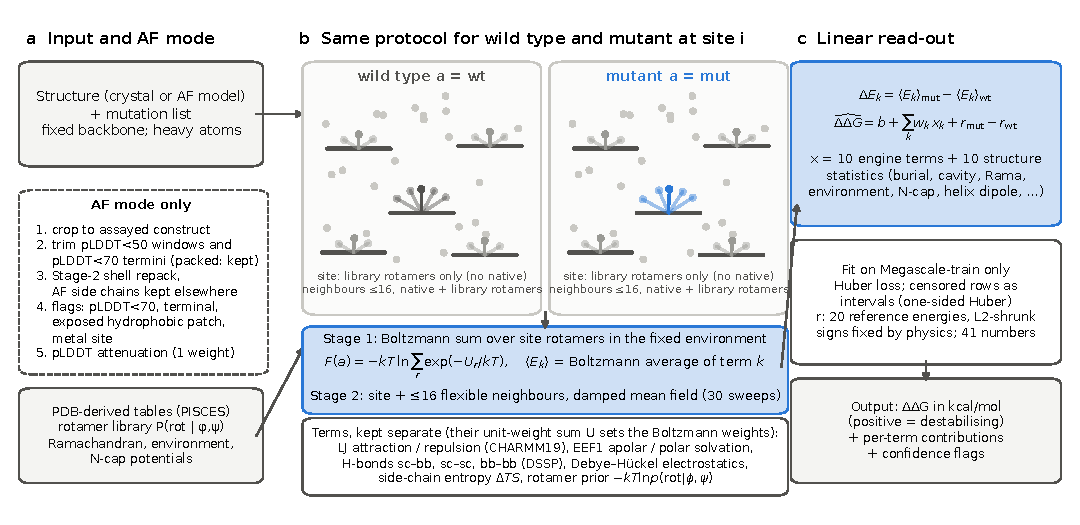
\includegraphics[width=\textwidth]{fig1_schematic.pdf}
\caption{How PhysDDG scores one mutation. The site is modelled with library rotamers only, identically for the
wild type and for the mutant, in the same structure; each identity is a Boltzmann ensemble, and the per-term
differences between the two ensembles enter a linear read-out. Stage 2 adds mean-field flexible neighbours. The
AlphaFold path changes the input and the reporting, not the energy function.}
\label{fig:schematic}
\end{figure*}

\subsection{Megascale}

On the 21 natural Megascale test proteins (22,159 variants, identical rows, identical AlphaFold2 structures) the
default model reaches a per-protein median $\rho$ of 0.692, against 0.629 for FoldX, 0.648 for the 10-weight
baseline, 0.622 for refitted tmol, 0.516 for DDGun3D and 0.500 for KORPM (Fig.~\ref{fig:megascale}a). The paired
difference to clipped FoldX is $+0.063$ with a 95\% cluster-bootstrap CI of $[+0.006, +0.120]$; it is $+0.062$
$[+0.009, +0.119]$ on the 14 homology-clean natural proteins and $+0.058$ $[+0.017, +0.121]$ on all 28. The
model ranks better than FoldX on 19 of the 21 proteins (Fig.~\ref{fig:megascale}b). Calibration separates the two
methods more clearly than ranking does: Pearson $r$ is 0.701 against 0.596 for clipped FoldX (paired $+0.105$,
CI $[+0.068, +0.135]$) and the RMSE is 0.776 against 1.845 kcal/mol. Against raw FoldX the Pearson difference is
$+0.256$, but most of that is the uncapped tail, so the clipped column is the fair one.

The AlphaFold variant is the best of our models on this set (0.699), and the fast Stage-1 model is the weakest
(0.678). Both differences are small. We note plainly that the shipped default is not distinguishable from the
previous rung of our own ladder: adding the N-cap and helix-dipole terms to the Stage-2 base is $+0.005$
$[-0.004, +0.019]$.

\begin{figure*}[t]
\centering
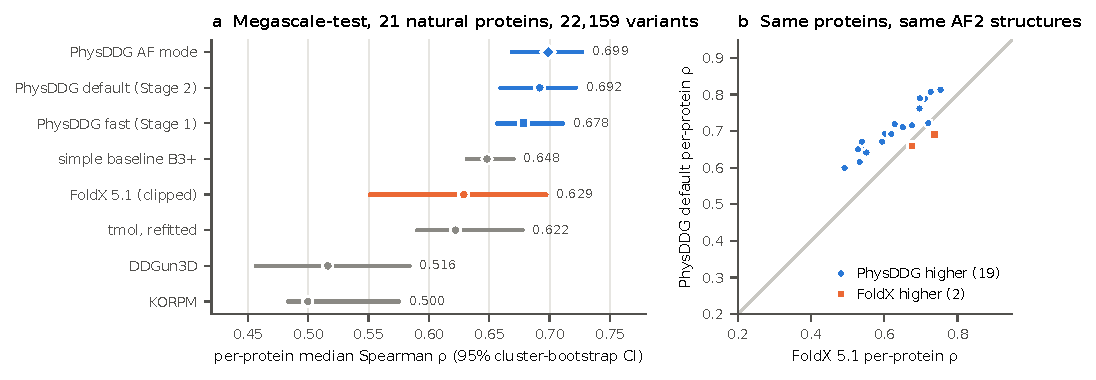
\includegraphics[width=\textwidth]{fig2_megascale.pdf}
\caption{Megascale test, natural domains. (a) Per-protein median Spearman $\rho$ with 95\% cluster-bootstrap
confidence intervals. (b) The same comparison per protein against clipped FoldX; the diagonal is equality.}
\label{fig:megascale}
\end{figure*}

\subsection{The other assays}

Table~\ref{tab:assays} and Fig.~\ref{fig:assays} give the per-assay picture, and it is much flatter. On FireProt
(347 rows, 27 proteins) the default model reaches $r = 0.451$ against 0.417 for clipped FoldX (paired $+0.036$,
CI $[-0.069, +0.102]$), 0.477 for refitted tmol and 0.488 for DDGun3D; no pair of methods separates on this set,
where the intervals are about $\pm 0.2$ wide. On S669-strict (488 rows) we reach 0.336 against 0.347 for DDGun3D
and 0.339 for the 10-weight baseline, and on S461-strict (290 rows) 0.552 against 0.570 for that baseline. In
other words the full engine buys nothing over ten descriptors on the crystal benchmarks. On Domainome the
default model is at 0.418 per-domain $\rho$ against 0.430 for FoldX (paired $-0.012$, CI $[-0.038, +0.021]$);
removing domains with a training homologue lowers every method by about 0.03 (ours 0.391, FoldX 0.385).

The joint variant, fitted on Megascale and FireProt together, is the better model on the abundance-type assays
(Domainome 0.450, strict 0.403) and on FireProt (0.478), at a visible cost on S669 and S461. It ships as an
alternative rather than as the default, because the family that wins on validation and cross-validation, the
only comparison that uses no test data, is the Megascale-only one (validation 0.7411 against 0.7297; grouped CV
0.6813 against 0.6648).

\begin{table*}[t]
\caption{Per-assay results. Megascale, Domainome and abundance: per-protein (per-domain) median Spearman $\rho$;
FireProt, S669 and S461: Pearson $r$. Each column is on the same rows for every model except where marked:
FoldX covers 341 and tmol 344 of the 347 FireProt rows, DDGun3D covers 47 of the 493 Domainome domains, and
the strict S669/S461/Domainome subsets of the joint variant are smaller because they also exclude FireProt
training homologues (470/285/320 rows or domains). Dashes mean the method was not run on that set. Confidence
intervals are in Supplementary Table S2.}
\label{tab:assays}
\small
\begin{tabular*}{\textwidth}{@{\extracolsep\fill}lccccccc@{}}
\toprule
model & Megascale nat & Megascale all & FireProt & S669-strict & S461-strict & Domainome & Dom.\ strict \\
 & 22,159 / 21 & 28,172 / 28 & 347 / 27 & 488 / 87 & 290 / 43 & 509,388 / 493 & 358,755 / 347 \\
\midrule
PhysDDG default (Stage 2) & \textbf{0.692} & \textbf{0.692} & 0.451 & 0.336 & 0.552 & 0.418 & 0.391 \\
PhysDDG fast (Stage 1) & 0.678 & 0.684 & 0.444 & 0.346 & 0.572 & 0.414 & 0.389 \\
PhysDDG AlphaFold mode & 0.699 & 0.699 & 0.451 & 0.336 & 0.552 & 0.425 & 0.397 \\
PhysDDG joint variant & 0.690 & 0.684 & \textbf{0.478} & 0.319 & 0.531 & \textbf{0.450} & \textbf{0.403} \\
Simple baseline B3+ (10 weights) & 0.648 & 0.649 & 0.432 & 0.339 & \textbf{0.570} & 0.389 & 0.369 \\
FoldX 5.1 raw / clipped & 0.629 & 0.633 & 0.411 / 0.417$^{\dagger}$ & -- & -- & 0.430 & 0.385 \\
tmol, 12 terms refitted & 0.622 & 0.626 & 0.477$^{\dagger}$ & -- & -- & -- & -- \\
KORPM & 0.500 & 0.533 & 0.397 & 0.194 & 0.543 & 0.302 & 0.274 \\
DDGun3D & 0.516 & 0.502 & \textbf{0.488} & \textbf{0.347} & 0.552 & 0.282$^{\dagger}$ & 0.282$^{\dagger}$ \\
\botrule
\end{tabular*}
\begin{tablenotes}
\item $^{\dagger}$ computed on a subset of the rows or domains of that column (see caption).
\end{tablenotes}
\end{table*}

\begin{figure*}[t]
\centering
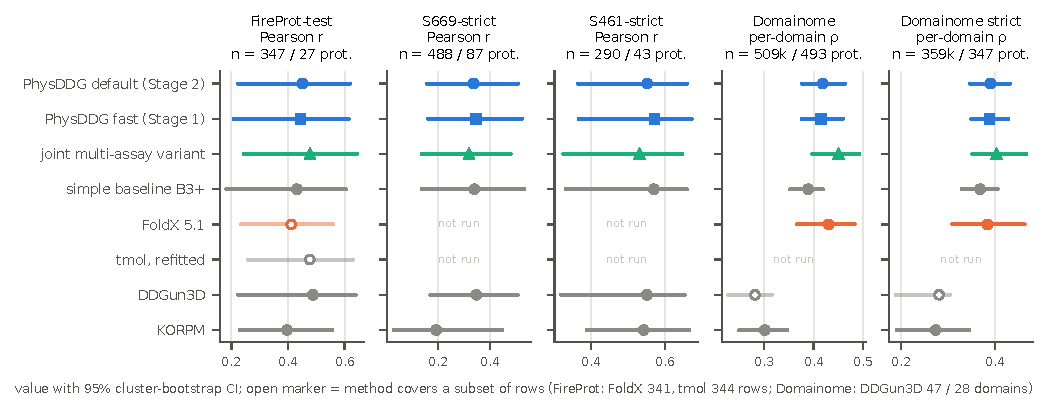
\includegraphics[width=\textwidth]{fig3_assays.pdf}
\caption{Per-assay values with 95\% cluster-bootstrap confidence intervals. Open markers mark methods that cover
only part of the rows of that panel. The intervals on the small crystal sets are wide enough that no pair of
methods separates there.}
\label{fig:assays}
\end{figure*}

\subsection{AlphaFold inputs}
\label{sec:af}

On the paired crystal/AlphaFold set (3,858 variants, 198 entities) the fitted models give nearly the same
prediction on either structure (per-entity median $r$ 0.95) and are no less accurate on the AlphaFold model
(Fig.~\ref{fig:af}b); the unfitted energy agrees much less (0.82 to 0.84) because the repulsion and side-chain
hydrogen-bond terms are sensitive to exact placement, and the fit already damps those terms. Where the two
structures differ most, the AlphaFold model is the better input for the unfitted energy ($+0.29$ Spearman at
local RMSD 0.6--1.0\,\AA{}); for the fitted models the same comparison has a confidence interval that includes
zero. Global repacking of all side chains makes agreement slightly worse, which reproduces
\citet{vangaru2025} in our own energy function.

Domainome is the low-confidence stress test. Accuracy falls with site pLDDT for every method and reaches zero
below pLDDT 70 (Fig.~\ref{fig:af}a): the default model has a per-domain median $\rho$ of 0.474 above pLDDT 90,
0.311 between 70 and 90, and $-0.013$ between 50 and 70. Most of that gradient is a burial effect, because
low-pLDDT sites are almost all exposed and every physics model is near zero at exposed sites at any confidence.
The useful response is to withhold rather than to correct: dropping the variants flagged as low pLDDT, terminal
or exposed hydrophobic patch, 14\% of rows, raises the per-domain median by 0.03 to 0.04, which is more than
every computational treatment we tried put together. The one correction that ships, pLDDT attenuation, has a
weight of $-0.97$ with a bootstrap interval that includes zero and gains $+0.012$ $[+0.006, +0.019]$ on
Domainome, so it is enabled for AlphaFold inputs only.

\begin{figure*}[t]
\centering
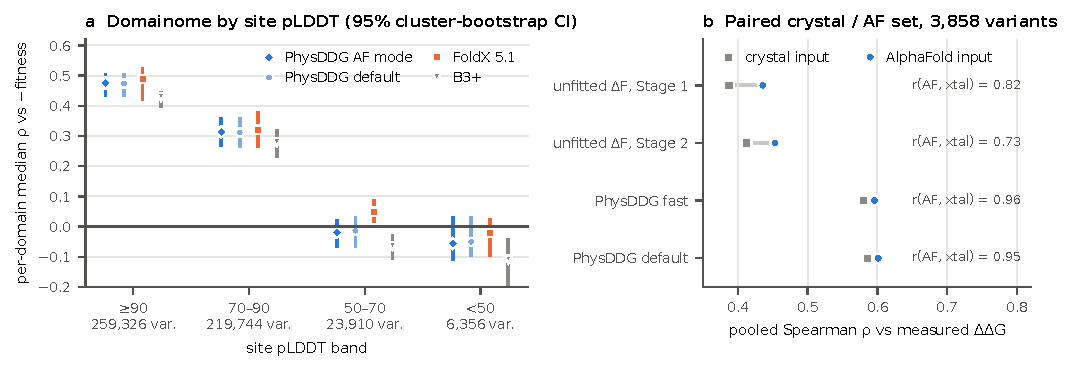
\includegraphics[width=\textwidth]{fig4_afmode.pdf}
\caption{(a) Domainome accuracy by site pLDDT band, with 95\% cluster-bootstrap intervals over domains with at
least 10 variants in the band. Every method is at zero below pLDDT 70. (b) On the paired set the fitted models
give the same answer on the crystal and on the AlphaFold structure; the unfitted free energy does not.}
\label{fig:af}
\end{figure*}

\subsection{What the terms contribute}

Every free weight carries the sign that physics predicts (Fig.~\ref{fig:terms}a), and the weights are all below
one, so the unit-weight energy sum is systematically too steep. The largest single weights are the cavity term
($1.086 \pm 0.133$ kcal/mol per unit) and burial ($0.916 \pm 0.077$); among the engine energies the largest are
backbone hydrogen bonds ($0.340$) and screened electrostatics ($0.343 \pm 0.045$). The environment potential
takes $0.221 \pm 0.018$ kcal/mol per $kT$ of log-odds, so the raw PDB statistics are about twice as confident as
the data supports.

Dropping one group at a time (Fig.~\ref{fig:terms}b) shows no dominant group. Removing the structure-derived
scalars costs 0.047 per-protein $\rho$ in cross-validation, removing all eight engine energies costs 0.032, the
reference energies 0.022, and each individual energy group between $-0.003$ and 0.011 (dropping the two
solvation terms alone improves cross-validation by 0.003). The engine is therefore not
redundant given the statistical potential, and the statistical potential is not redundant given the engine; the
two halves overlap heavily and each one carries signal. Going from Stage 1 to Stage 2 is worth 0.006 in cross-validation
and 0.014 on test, concentrated where it was predicted: on buried small-to-large substitutions, the stratum where
a fixed backbone fails, Stage 2 gains 0.034 pooled and 0.058 per-protein $\rho$ out of fold, in 5 of 5 folds.
Overall the repacking gain of 0.004 to 0.005 is far below the 0.02 we had pre-registered, so neighbour repacking
failed its gate and is kept only for that stratum and for AlphaFold inputs.

\begin{figure*}[t]
\centering
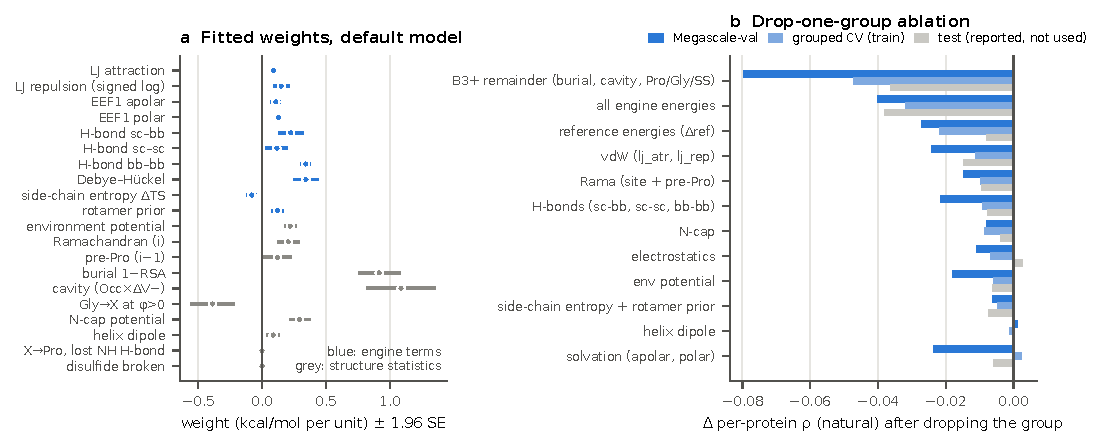
\includegraphics[width=\textwidth]{fig5_terms.pdf}
\caption{(a) Fitted weights of the default model with cluster-bootstrap intervals. (b) Change in per-protein
$\rho$ when one group of terms is dropped, on validation, in grouped cross-validation and on the test set (the
test column was computed after the decision and used for none of them).}
\label{fig:terms}
\end{figure*}

\subsection{Speed}

A full saturation scan on one RTX 4090, end to end including loading and feature computation, takes 0.9\,s for
59 residues, 3.6\,s for 269 and 10.0\,s for 597 in Stage 1, and 1.8 to 23.7\,s in Stage 2; the whole Domainome
set (532,000 variants) takes 71\,s in Stage 1 on four GPUs. FoldX needs 5 to 10 CPU-seconds per mutation, so the
comparison with FoldX is GPU-seconds against CPU-hours. Per mutation, however, we are only at parity with KORPM
(about 0.7\,ms on one GPU against 0.44\,ms on one CPU core), so speed on its own is not the contribution.

\subsection{Evolutionary information, kept separate}

A single extra weight on a sequence-profile log-ratio, computed with HHblits against UniClust30
\citep{steinegger2019} in the manner of DDGun \citep{montanucci2019}, raises the Megascale per-protein median
from 0.685 to 0.726 ($+0.040$, CI $[-0.005, +0.071]$) and Domainome from 0.411 to 0.486 ($+0.074$, CI $[+0.059,
+0.084]$). On the 14 homology-clean natural Megascale proteins the median change is $-0.006$ $[-0.037, +0.080]$
with a mean per-protein change of $+0.014$ and 9 of 14 proteins improving, so the Megascale gain is not
established on clean proteins. This mode is a different source of information and the alignment database
contains homologues of every natural benchmark protein, so we report it separately and keep it out of the
headline.

\subsection{Where the model is weak}

PhysDDG is not antisymmetric: on Ssym the correlation between the direct and the negated reverse prediction is
0.23 to 0.25 with a bias of $+1.4$ kcal/mol, against 0.88 for KORPM and 0.99 for DDGun3D. The defect is almost
entirely the repulsion term on a fixed backbone, where each crystal structure is relaxed around its resident
residue; no cap setting or transform that we tried removes it, and single-structure symmetrisation does not
either. A variant that drops the wild-type-site main effects reaches 0.59 at a cost of 0.044 per-protein $\rho$,
and we report it for use where antisymmetry matters. The model also ranks the top stabilising mutations worse
than FoldX (precision@5 0.15 to 0.23 against 0.219) although its AUROC for stabilising mutations is higher
(0.74 against 0.72); it is worse than FoldX on buried small-to-large substitutions (0.49 against 0.55); and it is
useless below pLDDT 70.

\section{Discussion}
\label{sec:disc}

What the evidence supports is one benchmark and two metrics. On Megascale, with identical rows and identical
structures, PhysDDG ranks mutations about 0.06 per-protein Spearman better than FoldX, with a confidence
interval from 0.01 to 0.12, and it is clearly better calibrated (Pearson 0.701 against 0.596; RMSE 0.78 against
1.85 kcal/mol). It does this at GPU-seconds per saturation scan and with 41 numbers fitted to $\Delta\Delta G$,
each of which has a physical reading and the physically expected sign.

What the evidence does not support is a claim of generalisation. On FireProt, S669, S461 and Domainome the model
is at the level of FoldX, and on the crystal sets the full engine does not beat a 10-parameter descriptor model.
The per-assay evidence stands on its own and we make no claim across assays. There is also a confound that we cannot
remove: all Megascale structures are AlphaFold2 models, so the benchmark on which the physics helps is also the
benchmark whose structures are predicted, and "physics helps on AlphaFold-based assays and adds nothing over
simple descriptors on crystal assays" is equally consistent with an assay effect and with a structure-source
effect. The paired crystal/AlphaFold set is the only experiment that separates the two, and it is small.

The headline rests on 21 proteins, of which 14 are homology-clean, and the FireProt per-protein median rests on
nine. We also did not keep the test sets untouched: counting from the version history, at least 12 evaluations
used test data and at least five of them changed what ships, including the decision to drop one site term and
two reversals after the second audit. With roughly 25 model variants and eight benchmarks, the selection
optimism on marginal differences is of the same size as those differences, so every delta below about 0.02 in
this paper should be read as suggestive. The validation and cross-validation numbers are the cleaner evidence,
and we report them next to the test numbers wherever a decision was made.

Finally, the model is not antisymmetric, which a physics model ought to be and which two much simpler methods
achieve. The defect is a single term on a fixed backbone. The obvious next step is backbone give at the site,
either as a directed local relaxation or as a learned per-site softening; random backbone ensembles, which we
tried, do not find the relevant relaxation (Supplementary Section S4).

\section{Key decisions}

Table~\ref{tab:decisions} lists the decisions that shaped the method and the reason for each. The full
decision log D1--D23, with dates and the evidence behind each, is in the repository.

\begin{table*}[t]
\caption{Decisions that shaped the method.}
\label{tab:decisions}
\small
\begin{tabular*}{\textwidth}{@{\extracolsep\fill}lp{0.23\textwidth}p{0.60\textwidth}@{}}
\toprule
ID & decision & reason \\
\midrule
D1 & positive $\Delta\Delta G$ = destabilising & FoldX convention; Megascale values flipped at ingestion after three independent sign checks \\
D2 & PyTorch as an array library only & no neural network and no pretrained model, while keeping GPU speed \\
D3 & own rotamer library from PISCES & the Dunbrack library needs a separate, manually approved licence and cannot be redistributed \\
D4 & environment statistical potential & the largest single omission found by the AI design reviewer; its $\sim$180 entries come from structures, not from $\Delta\Delta G$ \\
D5 & Boltzmann averaging over rotamers & suggested by the design reviewer; gives the entropy term for free and makes the objective smooth. On accuracy it is a wash against energy minimisation ($\pm 0.002$) \\
D6 & symmetric site modelling & library rotamers only at the site in both states; a wild-type to wild-type substitution must return exactly zero \\
D7 & shrunk reference energies with a dropped Megascale nuisance & the assay labels already contain an unfolded-state model, so part of the reference vector is assay-specific \\
D8 & censoring-aware loss & 11,363 strongly destabilising rows were excluded from the public table and re-enter as intervals \\
D9/D14 & site-dependent repulsion cap; repulsive radii $\times 0.9$ & fixed backbones over-penalise small-to-large substitutions; the radius scale was calibrated on structures, not on $\Delta\Delta G$. The cap setting turned out not to matter (spread 0.010 on validation) \\
D12 & fit on Megascale-train only; joint fit as a variant & decided on validation and cross-validation only, after the second audit reversed an earlier test-informed choice \\
D15 & terms must be state-function differences & wild-type-site-only terms break antisymmetry; they are reported as an ablation \\
D17 & reporting protocol & identical rows, strict subsets for S669/S461, FoldX raw and clipped, Ssym as a diagnostic only, paired bootstrap intervals for every comparison \\
D18 & flag rather than correct on AlphaFold inputs & withholding 14\% of variants gains more than every fitted correction together \\
D19 & drop the side-chain-contact term & it helps Megascale and Domainome but hurts all three crystal sets and transfers poorly between assays \\
D21 & elastic-network flexibility not adopted & the gain is a burial-dependent scale; a contact-number control recovers about 75\% of it \\
D23 & post-audit corrections & FireProt reported on all 347 rows; the disulfide term, determined by 8 rows, dropped; the 12 test evaluations disclosed; Domainome reported strict as well \\
\botrule
\end{tabular*}
\end{table*}

\section{Provenance of ideas}

The method is assembled from published ideas, and we name them. EEF1 implicit solvation and the CHARMM19
united-atom parameters are taken unchanged from \citet{lazaridis1999} and \citet{brooks1983,neria1996}. The
decomposition into separately weighted energy terms and the occupancy-style treatment of burial follow FoldX
\citep{guerois2002,schymkowitz2005}. From Rosetta we take the Lennard-Jones and solvation forms
\citep{alford2017,park2016}, the rotamer prior $-\log P(\mathrm{rot}\mid\phi,\psi)$ \citep{dunbrack1993}, the
orientation-dependent hydrogen-bond geometry of \citet{kortemme2003}, and the principle of
\texttt{cartesian\_ddg} that the wild type and the mutant undergo identical local protocols, which
\citet{valanciute2023} showed to be what keeps accuracy on model structures. Backbone-dependent rotamer
libraries are Dunbrack's idea \citep{dunbrack1993,shapovalov2011}; our library is derived independently from
PISCES-culled structures \citep{wang2003}. The split volume terms, the burial weighting and the
environment-dependent statistical potentials come from the PoPMuSiC line of work
\citep{gilis1997,dehouck2009}. KORPM \citep{hernandez2023} and DDGun \citep{montanucci2019,montanucci2022} are
our classical baselines, and the optional evolution mode uses DDGun's profile idea. The N-cap potential follows
the method of \citet{richardson1988} and the capping literature of \citet{doig1995}; helix-dipole and
helix-propensity ideas come from \citet{hol1978,shoemaker1987} and \citet{pace1998}. The unfolded-state
"mass-balance" reference energies are from \citet{rossi2025}, and the censoring treatment is dictated by the
assay model of \citet{tsuboyama2023}. The splits are ThermoMPNN's \citep{dieckhaus2024}; the benchmarks are
Domainome \citep{beltran2025}, ProteinGym \citep{notin2023}, S669/S461
\citep{pancotti2022,hernandez2023}, Ssym \citep{pucci2018} and FireProtDB \citep{stourac2021}. Trimming
low-confidence segments of AlphaFold models follows MAVISp \citep{arnaudi2026}, and keeping AlphaFold side
chains follows \citet{vangaru2025}. Secondary structure and backbone hydrogen bonds use the Kabsch-Sander
definition \citep{kabsch1983}; homology clustering uses MMseqs2 \citep{steinegger2017} and profiles use HH-suite
\citep{steinegger2019}. Mean-field and belief-propagation packing follow \citet{koehl1994} and
\citet{kamisetty2008}. tmol \citep{tmol} is our engine baseline. Three ideas in the final method, the
environment statistical potential, Boltzmann averaging over rotamers, and the censoring-aware loss, were
proposed by an AI reviewer that critiqued the design before it was built, and we say so explicitly.

\section{Data and code availability}

Code, the three shipped models, per-variant predictions for every benchmark, the decision log and both audit
reports are at \url{https://github.com/<OWNER>/physddg} (MIT licence for code, CC BY 4.0 for the predictions and
documents) and archived at Zenodo (DOI placeholder). The underlying measurements are public: Megascale
\citep{tsuboyama2023}, FireProtDB \citep{stourac2021}, S669/S461 \citep{pancotti2022,hernandez2023}, Ssym
\citep{pucci2018}, the Human Domainome \citep{beltran2025} and ProteinGym \citep{notin2023}. FoldX 5.1 requires
its own academic licence and the FoldX predictions used here are redistributed as numbers only. The figures in
this paper are produced by \texttt{manuscript/figures/make\_figures.py} from the result tables in the
repository.

\section{Acknowledgements}

This project was carried out by AI agents (Claude, Anthropic) under a human brief: one agent acted as principal
investigator and wrote the design, the research tree and the decision log; other agents curated the datasets,
implemented the geometry, energy, packing, fitting, prediction and evaluation code, ran the baselines and the
AlphaFold study, and produced two independent audits and two design critiques. The audits found and corrected
substantive errors in earlier versions of these results, including a row-dropping artefact in the FireProt
column and an undisclosed use of test data in model selection; both reports are released unedited. The human
owner supplied the brief, the data access and the compute. We thank the authors of the datasets and of the
competing methods for releasing their data and code.

\bibliographystyle{oup-abbrvnat}
\bibliography{references}

\end{document}
